\documentclass[a4paper, 11pt]{article}
\setlength{\topmargin}{-0.5in}
\setlength{\textheight}{9.5in}
\setlength{\oddsidemargin}{-.1in}
\setlength{\textwidth}{6.5in}

\usepackage{multirow}
\usepackage{float}
\usepackage{array}
\usepackage[document]{ragged2e}

\usepackage{datetime}

\newdateformat{mydate}{\monthname[\THEMONTH] \THEYEAR}

\newcolumntype{L}{>{\centering\arraybackslash}m{3cm}}

\usepackage{graphicx}
\graphicspath{{images/}}

\begin{document}


\LARGE\title{User Modeling in search for People with Autism}

\LARGE\author{Author: \textbf{Esha Massand}, Supervisor: \textbf{Keith Mannock}\\
\\
Birkbeck, University of London\\Department of Computer Science and Information Systems\\\\\\Project report submitted in partial fulfillment of the requirement for the MSc in Computer Science\date{\mydate\today}
\\\
}

\normalsize


\maketitle


\section*{Abstract}
\begin{justify}
This project report presents the development of a prototype web application to assist users with Autism when they search the web. The developed system models user interactions with the search process into a user profile by integrating insights from the core features of autism into the model. The user profile is applied to a synthesis of three leading search engines, and the entire system is integrated with an infra-red user interface component to assist users with Autism during search.\\
\end{justify}


\begin{justify}
This project is substantially the result of my own work, expressed in my own words, except where explicitly indicated in the text. I give my permission for it to be submitted to a Plagiarism Detection Service. This proposal may be freely copied and distributed provided the source is explicitly acknowledged.
\end{justify}

\begin{verbatim}














\end{verbatim}

\begin{center}
word count (proposal text only) : 3294 words.
\end{center}

\clearpage
\tableofcontents
\clearpage

\section*{Abbreviations}
\begin{tabular}{l l }
API & Application Programming Interface\\
AQ & Autism Quotient\\
ASD & Autism Spectrum Disorder\\
DSM & Diagnostic and Statistical Manual\\
GCS & Google Custom Search\\
HCI & Human Computer Interaction\\
HTTP & Hypertext Transfer Protocol\\
JSON & JavaScript Object Notation\\
IDE & Integrated Development Environment\\
KWIC & Key Word In Context\\
LEAP & LEAP Motion Controller\\
REST & Representational state transfer\\
RIFT & Oculus Rift Virtual Reality Head Mounted Display\\
TDD & Test Driven Development\\
UI & User Interface\\
UX & User Experience\\
VR & Virtual Reality\\
\end{tabular}

\section*{Definitions}

\begin{tabular}{l p{15cm}  }
Autism & Autism is amongst the most common neurodevelopmental condition and it is currently estimated that 1/68 children meet criteria for Autism Spectrum \cite{CDC}. Autism is five times more common amongst boys than girls (1/42 boys, and 1/189 girls). According to the Diagnostic and Statistical Manual (2013), Autism is characterized by persistent and early deficits in reciprocal social interaction and repetitive behaviours. Individuals vary from high functioning to low functioning (along a spectrum), with behaviours emerging around 2 to 3 years of age.
\end{tabular}
\clearpage

\section{Introduction}\label{intro}

This project report presents the development and evaluation of a prototype web-browser based application to assist users with Autism when they search the web, hereafter referred to as Jellibeans \footnote{Jellibeans are a rainbow of colours, different sizes and shades, and the name represents the difference in style of processing of individuals with ASD.}. Jellibeans will run in a web browser and utilises gesture and hand movement data recorded using the Leap Motion Controller (LEAP). 

Individual characteristics of each user will be measured using a 50 item questionnaire, the Autism Quotient (AQ \cite{Baron Cohen et al}) which measures tendency towards autistic traits. A score of 32 or higher indicates a strong likelihood of Autism or Asperger syndrome (the questionnaire has a 79\% sensitivity score). Individuals who score highly on the AQ will be offered the current user model for their search. The questionnaire data will be stored in the user's Google+ profile????

In programmatic terms, Jellibeans is designed to implement a research-based user model in search. This itself is a considerable part of the current research project and involves the development of a rule engine to transform the idiosyncratic ??? nature of search queries formed by individuals with ASD to work with current available search engines. This development involved collecting and analysing search behaviour patterns from people with and without ASD and building a set of transformation rules given the features of search queries that are formed by individuals with ASD.

Jellibeans will also improve the search experience for users with ASD by going one step further and enabling motion controlled search using the LEAP motion controller. The interface will be dynamic as opposed to static and this afford many advantages over traditional search engine interfaces.

\subsection {User Models in Search}

\subsection {Rule and Transformation Engine}

\subsection {Motion Controlled Navigation in Search}


\section {Aims}
The goal of the project is to build a prototype search tool that assists users with Autism search and navigate the web. To acheive this goal, the aims of this work are:

To synthesise the search results from three search engines, Google, Bing and Yahoo. For search results returned by Google, the Custom Search API will be used in line with the Google terms of service (as `screen scraping', or copying the data directly from the website is prohibited). It is a RESTful api with a single method called list. The API method used was GET, and the response data is returned as a JSON type. The response consists of (1) the actual search result, (2) metadata for search like number of  results, alternative search queries, and (3) custom search engine metadata. The data model depends on \cite{opensearch}.
For Bing and Yahoo search results, JSoup (a Java HTML parser) will be used to identify the links from the resulting query. The JSoup HTML parser was considered more effient for retrieving search results, as it reduced the number of lines of code required to complete the task. 
Jsoup has its advantages over html parsing. It contains a class representing a list of nodes, `Elements', which implements Iterable to iterate over a list in an enhanced for loop.
The resulting links are written to text file which stores the links in a text file in the projects source directory.


To build a stereotyped user model (a user model that will infer characteristics about the user from their diagnostic information) for a person with ASD. Users will have to register will Google+, and report their diagnostic information in the aboutMe section of their profile. Using the Google+ API, Jellibeans will connect to Google+ and ask the user to signin/ agree to the web application accessing their data. JavaScript will be used to parse the text in the aboutMe section to check if the user has identified as a persn with autism, aspergers, ASD or not. The result is returned via the console (inspect) command.


\section {Method}
\subsection{Building the User Model}\label{building the user model} 
There are many stages to the search process. After identifying the information need, the user must formulate a search query. The user must browse through results once the query has been entered into a search engine. The whole process can be repeated if the user is not satisfied. The stage at which the user model will have most possible impact is before results are returned to the user, that is, at the query formulation stage. It is this stage that the user model will be implemeted (stage 2 on Figure~\ref{search flow}).

\begin{figure}[H]
\begin{center}
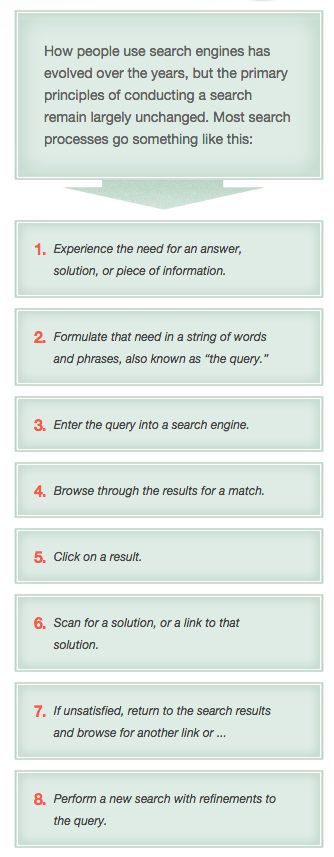
\includegraphics[scale=0.6]{tdSearch}\\
\caption{Typical user's search flow process \cite{seo}}
\label{search flow}
\end{center}
\end{figure}

Search queries usually fall into one of three broad categories.  `Do" queries which characterise transactions between the user and the search engine, for example when the user wants to do something such as buy a plane ticket or listen to a song. There are also `Know" type queries. These are informational queries for example, the name of a band or restaurant in London. The third broad category is `Go" type queries, which are navigational in nature, for example, searching for a particular home page on the web. 



\subsection{Differences in Search Queries Between Users With and Without Autism}
The primary goal of the search engine is to deliver relevant results to the user, but what is `relevant"? Not all users or groups of users search in the same way, so it is important to consider user intentions. The first part of the current project aimed to investigate the differences between search queries of people with and without Autism. 

\subsection{User requirements}
\subsection{User behaviours}
\subsection{Design of user model}


\subsection{Implementation}
What was actually done
From theoretical to concrete
Results of the data collection
Profile of users and user groups
Classification of users
Feature uses
Storage of information


\subsubsection{Integrating Jellibean with Motion Controller Hardware}
LEAP motion controller and its use for the system.
Current Project’s Hardware Selection Process and Important Design Issues:
\begin{enumerate}
\item{Good timing correlates to a good meaning and User Experience.}
\item{The leap has options to ‘poll’ frames at a constant rate (to keep timing of movement accurate) which is important.}
\item{Cognitive ‘lag’ time. Each of our senses operates with a different lag time. Hearing has the fastest sense-to-cognition/understanding time, and surprisingly sight -- the slowest. If the devices interferes with the processing of the sense, it will confuse the combinatorial configuration of the senses, leading to misunderstandings in the meaning and a worse user experience.}
\item{Volume is important because this is a tool to be used with individuals with ASD, the device must have a low `volume’, i.e., the sensory experience cannot be overwhelming.}
\item{Load, by this I mean `cognitive' load is most desirable when not high. We do not want the device to be overwhelming in terms of it’s cognitive load.}
\item{Within the selection process, I did not just consider the physical design of the device, but also the way in which the devices manifests actions into behaviours. That is, how does the user engage behaviourally within the environment using the device? What about the physical sensation and its path towards a behavioural or emotional response? For example, can we program there to be an activity followed by a reward to reinforce the activity.}
\end{enumerate}


\subsection{Development and Implementation of Jellibean}
\subsection{API's and Development Tools}


\section{Result}
The transformations that were implemented


\section{Conclusion}
How does it compare to the original specification
This work has successfully completed aims XXX

\subsection{Signals of Quality Content}
I will test and evaluate the system. Testing will involve assessing the reliability and robustness of Jellibeans; the ease of its interaction; boundary conditions; ease of use; does it fullfil the aims of the project.
Evaluation of the system will include comparisons to existing search engines; assessing how this idea can be implemented to tailor an existing systems; assessing how well the system does compared to existing systems on a set of criteria that are only relevant to the user group in question (a collective measure of user happiness). Evaluation will also include quantitative metrics such as Recall, Precision, and False Negative/Positive rates.


Apache Solr


	

\section {Critical Review of the Leap Motion Controller}
Advantages
\begin{enumerate}
\item{Impressive}
\item{Uses infrared to embed the users (phantom) hand™ on the screen}
\item{New technology and novel to bring to laptops}
\item{East to set up}
\item{Has built in gestures and navigation tools}
\item{Can work in pretty dimly lit environments (but not all)}
\item{It is sophisticated (sometimes the polling frequency lets it down)}
\item{Picks up an impressive distance along the z axis}
\item{Offers a recalibration process if the controller is persistently jumpy, or there are discontinuities in the tracking data, if there are aberrations in the tracking data that occur in certain areas of the field of view, or poor tracking range. This can be done using the shiny surface such as the computer screen or mirror.}
\end{enumerate}	
Disadvantages
\begin{enumerate}
\item{Misses small hand movements}
\item{The range that it will detect is 150 degree angle along the y axis, this is reasonable but not always idea when gestures/hand movements are large.}
\item{Some parts of the screen the hands to not ‘reach’, i.e., bottom left /right of screen are sometimes hard to reach.}
\item{Loses the hand, stops working/sensing the hands, even when the controller stays on.}
\item{Often misses frames, so the user makes larger hand movements and then overshoots (when the LEAP catches up)}
\item{Built-in controls are not ideal}
\item{Lighting works best when the hand is seen in silhouette fashion by the controller. }
\end{enumerate}




\clearpage
\begin{thebibliography}{100}
\bibitem{Baron Cohen et al} Baron-Cohen, Wheelrigjt, Skinner, Martin, Clubley (2001).   The Autism-Spectrum Quotient (AQ): evidence from Asperger Syndrome/high-functioning autism, males and females, scientists and mathematicians.  Journal of Autism and Developmental Disorders, 31, 5-17.
\bibitem {opensearch}OpenSearch, http://www.opensearch.org/Specifications/OpenSearch/1.1, Retrieved 30 July 2015.
\bibitem{seo} Fishkin (2015) https://moz.com/beginners-guide-to-seo/how-people-interact-with-search-engines, Retrieved 3 August 2015.
\end{thebibliography}
\end{document}